\section{Arquitectura Delta}


La Arquitectura Delta surge desde Databricks, al igual que la Arquitectura Kappa, 
como una respuesta a los desafíos que presenta la arquitectura Lambda.
A diferencia de la suposición que hace Kappa de que todo puede ser tratado como un Stream, 
Delta por su parte, utiliza el almacenamiento de objetos en la nube como sustrato de almacenamiento y 
agrega por encima tecnología de metadata que otorga la posibilidad de utilizar este sistema de almacenamiento
como un canal de mensajes de modo que se puede hacer Streaming sobre él; además de agregar otras capacidades.
Esto permite utilizar una única tecnología tanto para análisis en tiempo real como análisis histórico. 


\subsection{Descripción General}

Delta parte de la premisa de que es deseable separar la capacidad de cómputo de la capacidad de almacenamiento; 
y que además es deseable hacerlo en base a sistemas de almacenamiento de objetos en la nube ya que son extremadamente
baratos y escalables. 

El desafío es entonces, alcanzar un almacenamiento que tenga buen rendimiento y que permita ser mutable sobre
este tipo de sistemas. Como se describió previamente, estos sistemas de almacenamiento tienen dificultades
en cuanto a la correctitud y el rendimiento en cuanto se intentan mutar multiples objetos a la vez. Un ejemplo
podría ser, la actualización del dataset entero para un usuario por cuestiones de normativa como GDPR.

La solución a este tipo de problemas, es un formato de tabla analítica sobre el almacenamiento subyacente. 

\newpage
\subsection{Componentes Principales}

\subsubsection{Formato de Tabla Analítica}

Los formatos de tabla analítica son tecnologías diseñadas para resolver los desafíos del manejo de datos
a gran escala. Surgen como respuesta a las limitaciones de los formatos de archivo tradicionales como Parquet y ORC
cuando se trabaja con ellos en la nube. 

Las características más importantes que aporta un formato de tabla analítica son:
\begin{itemize}
    \item Soporte para transacciones ACID
    \item Control de versiones en los datos
    \item Capacidad de realizar operaciones de actualización y eliminación múltiples
    \item Compatibilidad con múltiples motores de procesamiento
\end{itemize}

Los formatos de tablas analíticas dan a sus sistemas subyacentes estas características a través de diferentes mecanismos y estrategias. 
La principal es la gestión de metadatos, ya que implementan estructuras de datos altamente optimizadas que permiten rastrear 
eficientemente los archivos y sus cambios; mientras mantienen un historial detallado de transacciones que garantiza la consistencia de los datos, 
complementando con estrategias efectivas de particionamiento y organización. 

Para la optimización del rendimiento, estos formatos emplean diversas técnicas como la compactación automática de archivos, 
estrategias de caching de datos para acceso rápido, utilización de formatos de archivo columnares como Parquet u ORC, 
y la incorporación de capacidades avanzadas de indexación y filtrado optimizado. 
La consistencia de los datos se garantiza mediante la implementación de transacciones ACID completas, 
que proporcionan un sólido aislamiento entre operaciones de lectura y escritura, manejan conflictos de manera automática 
y aseguran la consistencia en escenarios de operaciones concurrentes. 
En cuanto a la evolución y mantenimiento, estos formatos facilitan cambios de esquema sin interrupciones en el servicio. 

Todas estas mecanismos trabajan en conjunto para proporcionar una solución completa para el manejo de datos a escala masiva,
que como subproducto permite tratar la escritura de los archivos como un canal de mensajes sobre el que se puede hacer streaming.

Los exponentes más importantes de estos formatos son: Delta Table, Apache Iceberg y Apache Hudi


\subsubsection{Delta Lake}

Delta Lake (diseñada por Databricks) implementa una arquitectura de almacenamiento que se construye sobre archivos Parquet como formato base, 
organizándolos en una estructura de directorios. 
Cada tabla Delta está compuesta por dos elementos fundamentales: los archivos de datos en formato Parquet y el directorio {\_delta\_log} 
que contiene los metadatos y el registro de transacciones. 
Esta estructura permite mantener las ventajas de rendimiento y compresión eficiente de Parquet 
mientras añade capacidades transaccionales y de control de versiones.

El {\_delta\_log} representa el componente central que permite mantener el control de versiones y garantizar las propiedades ACID. 
Funciona como un registro detallado de cambios donde cada modificación se almacena en archivos JSON numerados secuencialmente. 
Cada uno de estos archivos contiene una o más acciones como añadir o eliminar archivos, actualizar metadatos, entre otras operaciones. 
Las transacciones se registran de forma atómica mediante operaciones del sistema de archivos, 
permitiendo reconstruir el estado exacto de la tabla en cualquier momento consultando este historial de cambios.

Para optimizar el rendimiento, se implementa un sistema de checkpoints que se generan automáticamente 
cada cierto número de transacciones. 
Estos checkpoints contienen una imagen completa del estado de la tabla en formato Parquet, 
evitando la necesidad de procesar todo el log desde el inicio al leer la tabla. 
Incluyen información crucial como la lista de archivos válidos, el esquema actual, la configuración de particionamiento 
y estadísticas detalladas de la tabla, funcionando como puntos de referencia rápidos para acceder al estado de la tabla.

El manejo de concurrencia se realiza a través de un sistema que combina control de concurrencia optimista con serialización de escrituras. 
Este enfoque permite que múltiples lectores y escritores trabajen simultáneamente mientras mantiene la consistencia de los datos. 
Las lecturas operan bajo "snapshot isolation", garantizando que cada lector vea una versión consistente de los datos,
mientras que las escrituras se serializan mediante un protocolo no bloqueante 
que utiliza operaciones atómicas del sistema de archivos para coordinación. 
El sistema incluye lógica de reintento automático para manejar conflictos de manera elegante.

Las características principales de Delta Lake incluyen transacciones ACID completas que garantizan consistencia en todas las operaciones, 
capacidades de acceder a versiones anteriores de los datos y volver atrás cuando sea necesario, 
y un sistema de evolución de esquema que previene la corrupción de datos. 
Las operaciones de Merge (UPSERTS) son particularmente sofisticadas, 
permitiendo actualizaciones eficientes de registros existentes con soporte para operaciones incrementales y condiciones de merge personalizables.

La optimización de datos es automática y tiene múltiples mecanismos, 
incluyendo compactación de archivos pequeños, optimización de consultas, y mantenimiento de estadísticas detalladas 
para mejor planificación de consultas. 

El soporte para streaming proporciona procesamiento de datos en tiempo real con semántica exactly-once y control de carga.

También presenta una excelente integración con Spark, aunque no tanto otros motores de procesamiento.

\subsubsection{Apache Hudi}

Apache Hudi (diseñado incialmente por Uber) implementa un sistema de almacenamiento que ofrece dos tipos principales de tablas: 
Copy On Write (COW) y Merge On Read (MOR). 
Las tablas COW almacenan datos directamente en formato columnar Parquet, donde cada actualización genera nuevas versiones de los archivos completos, 
optimizando así las lecturas pero con un mayor costo en escrituras.
Por otro lado, las tablas MOR utilizan un enfoque híbrido que combina archivos base en formato Parquet con archivos delta en formato Avro 
para los cambios recientes, proporcionando un balance entre rendimiento de lectura y escritura.

La gestión de metadatos se realiza mediante una Timeline que registra cronológicamente todas las acciones en una tabla. 
Estas incluyen COMMIT para nuevas inserciones o actualizaciones, {DELTA\_COMMIT} para escrituras en archivos delta en tablas MOR, 
CLEAN para limpieza de versiones antiguas, COMPACTION para la fusión de archivos delta con archivos base, RESTORE para rollbacks 
y SAVEPOINT para marcar puntos de recuperación específicos. 
Cada acción en la Timeline tiene un instant time único y mantiene metadatos detallados que permiten reconstruir el estado de la tabla 
en cualquier momento.

Para optimizar las operaciones, Hudi implementa un sistema de indexación versátil que incluye diferentes tipos de índices 
para búsquedas rápidas y la posibilidad de implementar índices personalizados. 
Esto facilita la localización eficiente de registros, optimiza las operaciones de upsert, 
maneja la deduplicación de datos y permite un ruteo optimizado de las escrituras.

Las características principales de Hudi incluyen un sistema de procesamiento incremental que permite manejar streams de datos incrementales, 
junto con consultas incrementales eficientes. 
El control de concurrencia se maneja a través de un control de concurrencia optimista que mantiene las lecturas sin bloqueos mientras 
serializa las escrituras para mantener la consistencia. 
Además, Hudi implementa características como gestión de compactación automática configurable, 
y un sistema de limpieza que mantiene el almacenamiento optimizado.

El manejo de registros individuales en Hudi es particularmente sofisticado, ofreciendo versionado a nivel de registro, borrado lógico, 
evolución de esquemas y actualizaciones a nivel de fila. 
Todo esto se mantiene bajo fuertes garantías de consistencia que incluyen transacciones ACID y semántica exactly-once. 

También presenta una muy buena integración con diferentes motores de procesamiento como Spark y Flink.

\subsubsection{Apache Iceberg}

Apache Iceberg (diseñado inicialmente por Netflix) implementa una arquitectura de almacenamiento que se distingue por su 
modelo de metadatos y su enfoque en la evolución del esquema. 
El formato utiliza una estructura de tabla que separa completamente los metadatos de los datos, 
manteniendo varios niveles de manifiestos que rastrean todos los archivos de datos. 
Esta jerarquía de metadatos incluye un archivo de metadatos principal, manifest lists que agrupan archivos de manifiesto, 
y manifiestos individuales que rastrean los archivos de datos. 
Los datos en sí se almacenan en formatos como Parquet o ORC, permitiendo una optimización efectiva para consultas analíticas.

El sistema de control de versiones de Iceberg se implementa a través de un modelo de snapshots atómicos. 
Cada snapshot representa un punto en el tiempo inmutable de la tabla y contiene referencias a todos los archivos de datos válidos para esa versión. 
Los snapshots se encadenan entre sí, formando un historial lineal de la tabla, permitiendo ir hacia atrás en el tiempo. 
Este diseño facilita las operaciones concurrentes y garantiza la consistencia sin necesidad de bloqueos pesados, 
ya que cada operación de escritura crea un nuevo snapshot sin modificar los existentes.

La gestión de esquemas en Iceberg permite evolucionar tanto el esquema de la tabla como la estrategia de particionamiento 
sin necesidad de reescribir datos. 
El sistema mantiene un historial de esquemas y asigna identificadores únicos a cada campo, 
permitiendo cambios seguros como añadir, renombrar o reordenar columnas. 
El particionamiento es tratado como metadatos, lo que permite cambiar la estrategia de particionamiento sin mover datos, 
una característica única que facilita la optimización continua del rendimiento de las consultas.

La optimización de consultas en Iceberg se beneficia de su capa de metadatos. 
El formato mantiene estadísticas detalladas a nivel de columna y archivos, 
incluyendo valores mínimos y máximos, conteos de nulos y otros metadatos que permiten una poda eficiente de particiones 
y archivos durante la planificación de consultas. A
demás, implementa características como la posibilidad de realizar lecturas incrementales eficientes, 
filtrado de datos a nivel de manifiesto, y soporte para operaciones de reescritura de datos optimizadas.

El control de concurrencia en Iceberg utiliza un enfoque optimista basado en la inmutabilidad de los snapshots. 
Las operaciones de lectura siempre ven una vista consistente de la tabla basada en un snapshot específico, 
mientras que las escrituras compiten por crear el siguiente snapshot en la cadena. 
Los conflictos se detectan y resuelven al momento del commit, y el sistema proporciona garantías de aislamiento y consistencia 
sin requerir un sistema de bloqueo centralizado.

Las características de mantenimiento incluyen la expiración de snapshots antiguos, compactación de archivos pequeños, 
y reescritura de datos para optimización física. 
Estas operaciones se pueden realizar de manera concurrente con las operaciones normales de lectura y escritura.

La integración con diferentes motores de procesamiento es otro punto fuerte ya que proporciona APIs nativas para Spark, Flink, y otros motores, 
permitiendo que cada motor optimice su acceso aprovechando las características avanzadas de metadatos y estadísticas.

\subsection{Vista Lógica}

\begin{figure}[h]
\centering
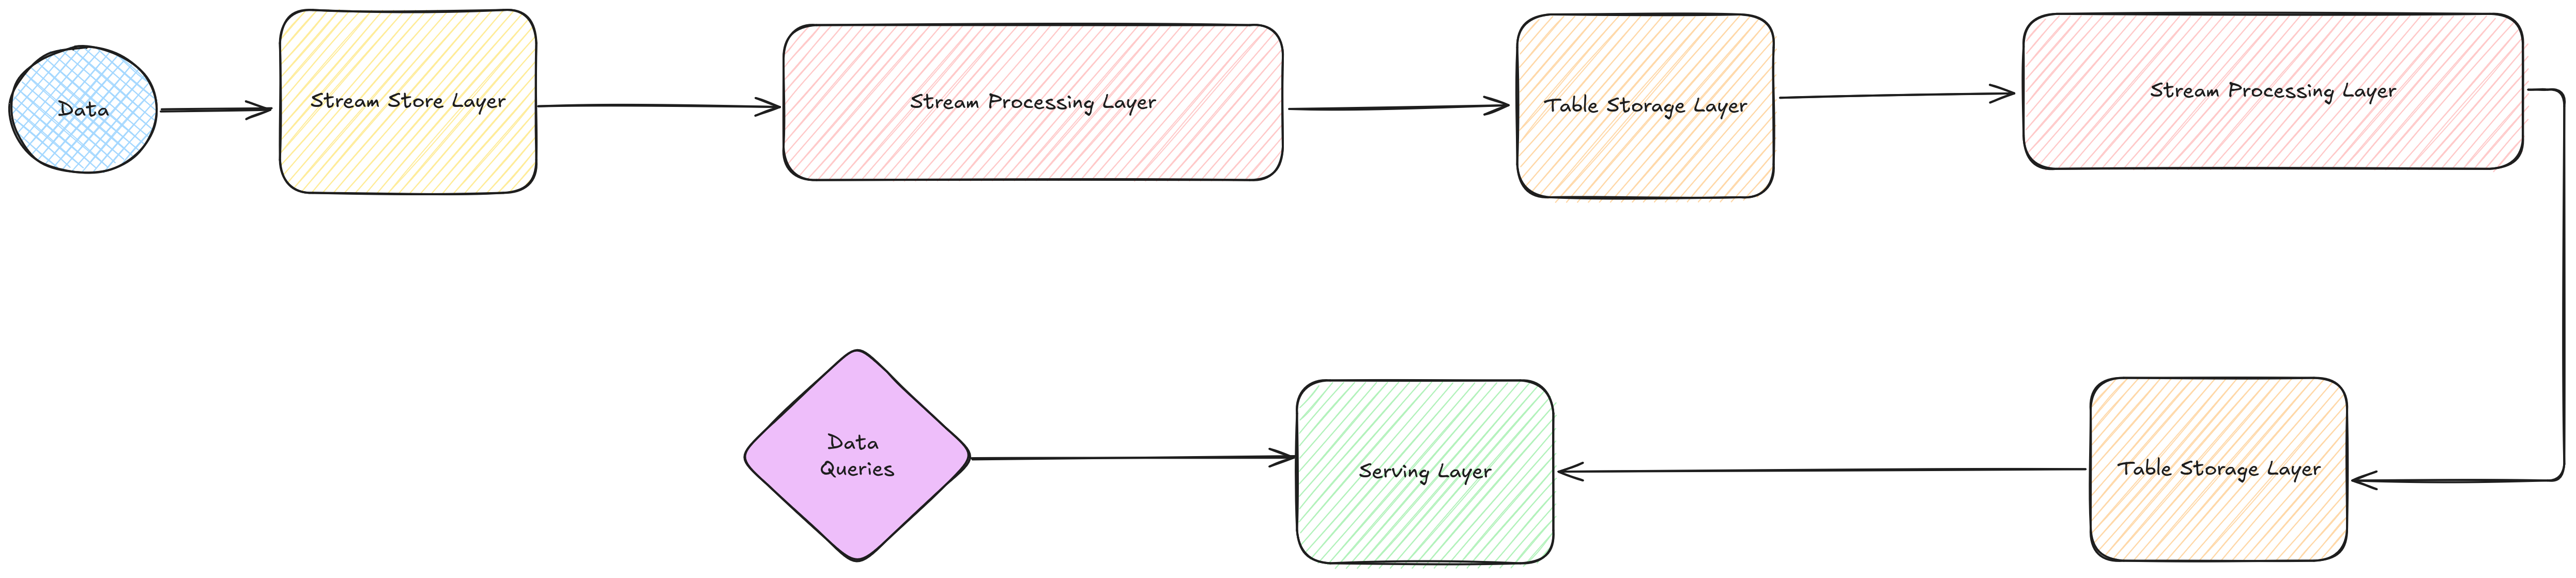
\includegraphics[width=0.8\textwidth]{teorico/delta.png}
\caption{Diagrama de la Arquitectura Delta}
\label{fig:arquitectura_delta}
\end{figure}

\subsection{Implementación Típica}

\subsection{Capacidades}

\subsection{Desafíos}
